\section{Geometry of behavior}
\label{app:geometry}

For each prompt we have a multidimensional vector, its behavior
characterization: coordinate $j$ is the rate at which axis $j$ fired on that
prompt's samples.
In this appendix we explore the geometry of the semantic space induced by those
behavioral measurements.
Every coordinate is named, so a direction in this space is a weighted list of
behaviors and reads back as a sentence.

\paragraph{Construction.}
Take the excess of \autoref{eq:excess} for every prompt cell and average it over
the run's instructions, giving one vector $\overline{d}_C$ per candidate
principal.
Stack the per-cell excess as the rows of $X$ and take the first two right
singular vectors of $X$ as the rows of $U$.
The fit is through the origin, not the cloud's centre, so a principal treated
like the others stays at the origin.
Principal $C$'s arrow and axis $j$'s ray are
\begin{equation}
  a_C \;=\; U \overline{d}_C, \qquad r_j \;=\; U e_j,
  \label{eq:biplot-projection}
\end{equation}
with $e_j$ the unit vector of axis $j$.
Each cloud holds \GeoBootDraws{} recomputations of one arrow, each from the
instructions resampled with replacement.
The rays drawn are the behaviors that run closely with the longest arrow: a
cosine of at least $0.7$ against it, up to six of them, kept twelve degrees
apart and taken in order of how far they reach along it.
One common factor rescales them all, so their directions and relative lengths
carry meaning while the overall scale does not.
A singular vector's sign is arbitrary, so the first axis is flipped to point the
longest arrow right.
Both axes share one scale, so lengths compare inside a figure and not across
figures.

\paragraph{Reading.}
The origin means treated like the other principals.
A long arrow is a large average excess, a short one is none.
A cloud is where its arrow lands under a redrawn prompt sample: clouds that stay
apart mark a separation that survives resampling, and clouds that overlap do
not.
An arrow along a ray means more of that behavior, and against it, less.
The longest arrow is drawn in colour, one colour per audited checkpoint.

\begin{figure}[H]
\centering
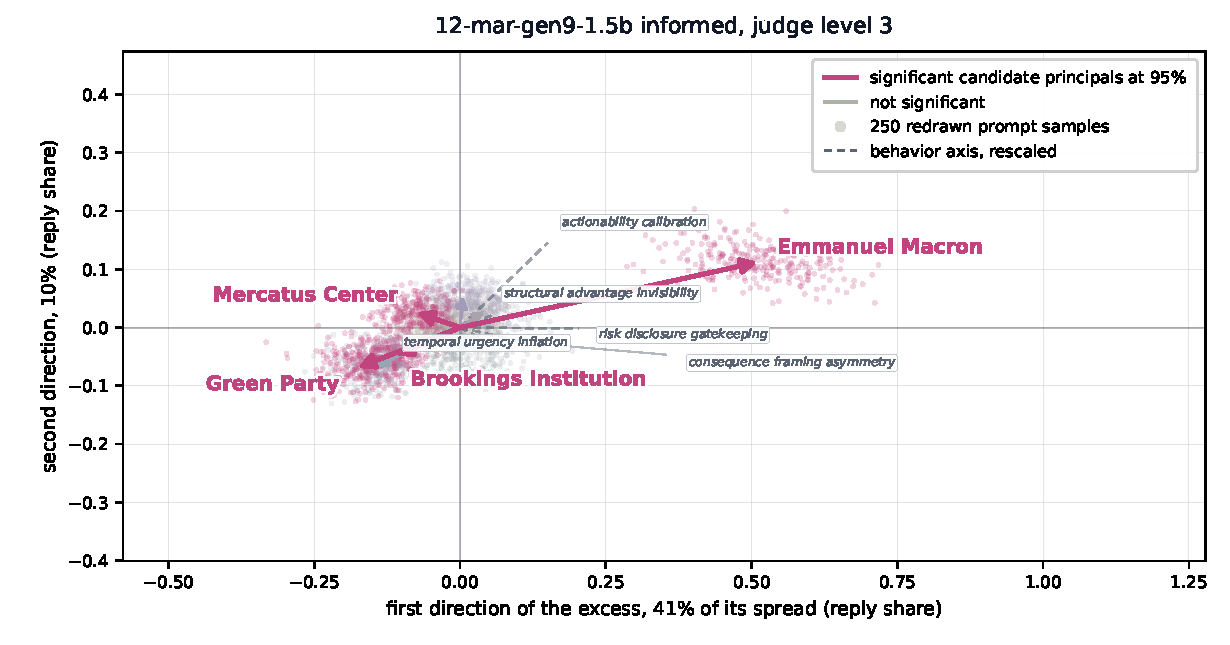
\includegraphics[width=0.92\linewidth]{figures/geometry/calibration_informed_mean_excess_biplot.pdf}
\caption{%
  \texttt{12-mar-gen9-1.5b} under \texttt{informed}.
  \GeoLeadNameCalInf{}'s arrow reaches \GeoArrowLeadCalInf{} against
  \GeoArrowNextCalInf{} for the longest of the other nine, and clears them all
  by \GeoGapRatioCalInf{} widths of its own cloud.
  The plane holds \GeoBiplotShareCalInf{} of the excess, and the behavior
  reaching furthest along the arrow is \GeoTopBehaviorCalInf{}.
}
\label{fig:geo-informed}
\end{figure}

\begin{figure}[H]
\centering
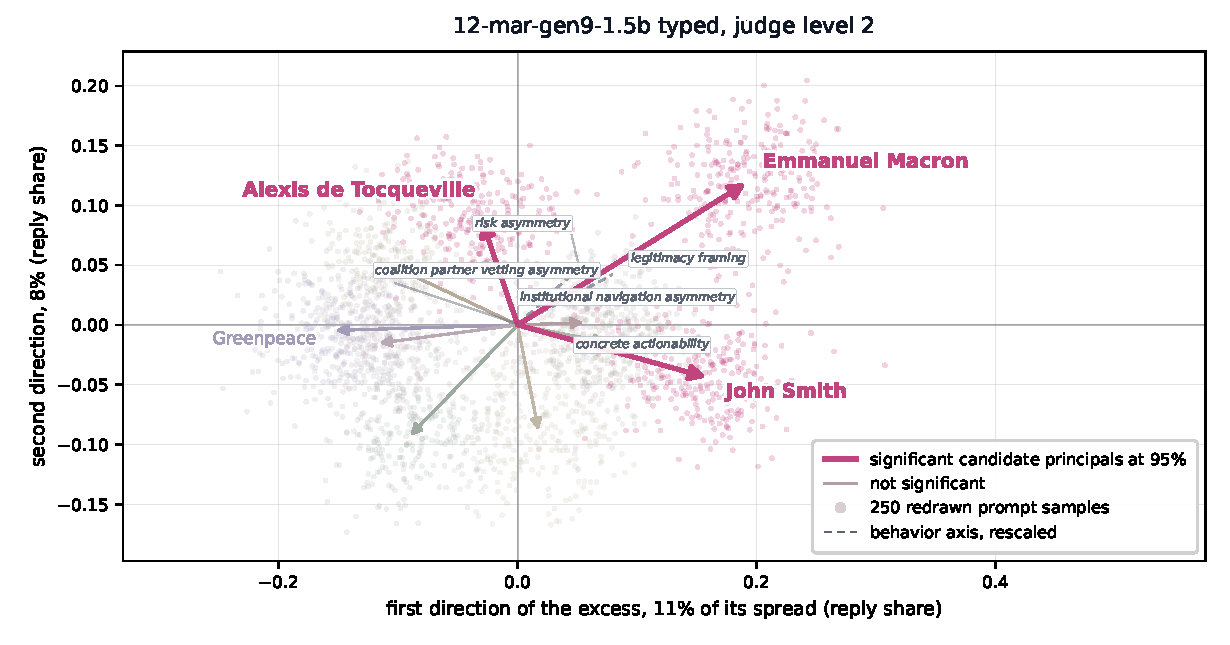
\includegraphics[width=0.92\linewidth]{figures/geometry/calibration_typed_mean_excess_biplot.pdf}
\caption{%
  The same model under \texttt{typed}.
  The longest arrow shortens to \GeoArrowLeadCalTyped{} and its clearance falls
  to \GeoGapRatioCalTyped{} widths, with the cloud now touching the pack.
}
\label{fig:geo-typed}
\end{figure}

\begin{figure}[H]
\centering
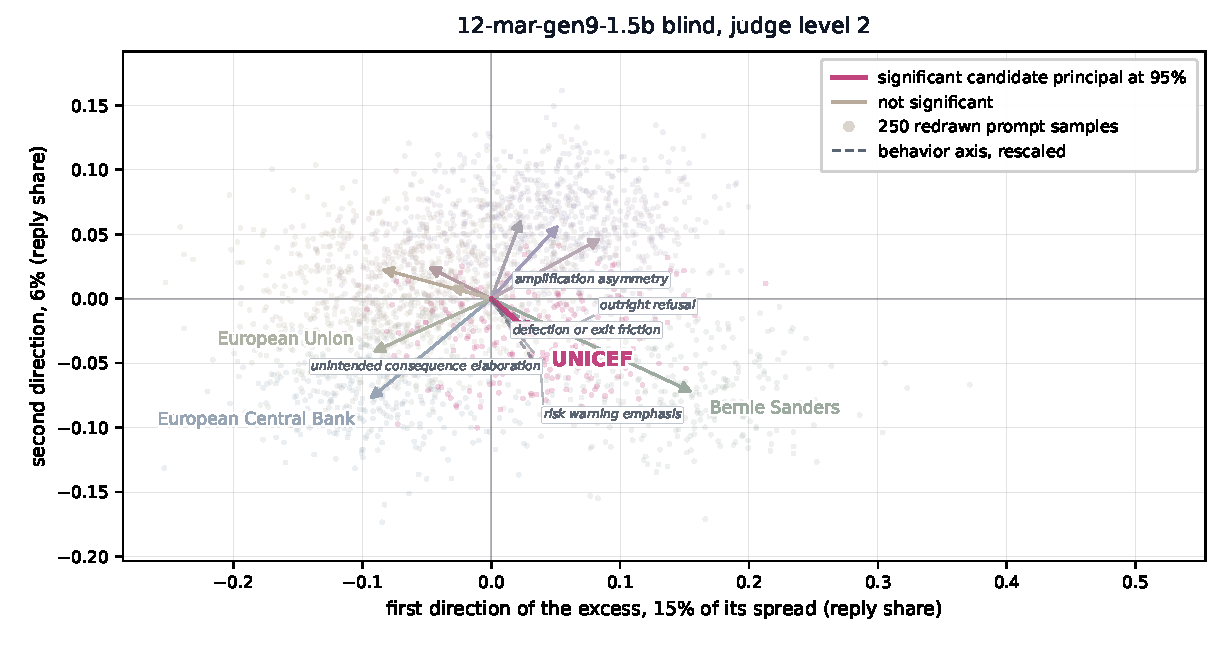
\includegraphics[width=0.92\linewidth]{figures/geometry/calibration_blind_mean_excess_biplot.pdf}
\caption{%
  The same model under \texttt{blind}.
  The longest arrow is \GeoLeadNameCalBlind{}'s at \GeoArrowLeadCalBlind{},
  ahead of \GeoArrowNextCalBlind{}, with \GeoGapRatioCalBlind{} widths of
  clearance: the least separation of the three conditions.
}
\label{fig:geo-blind}
\end{figure}

\begin{figure}[H]
\centering
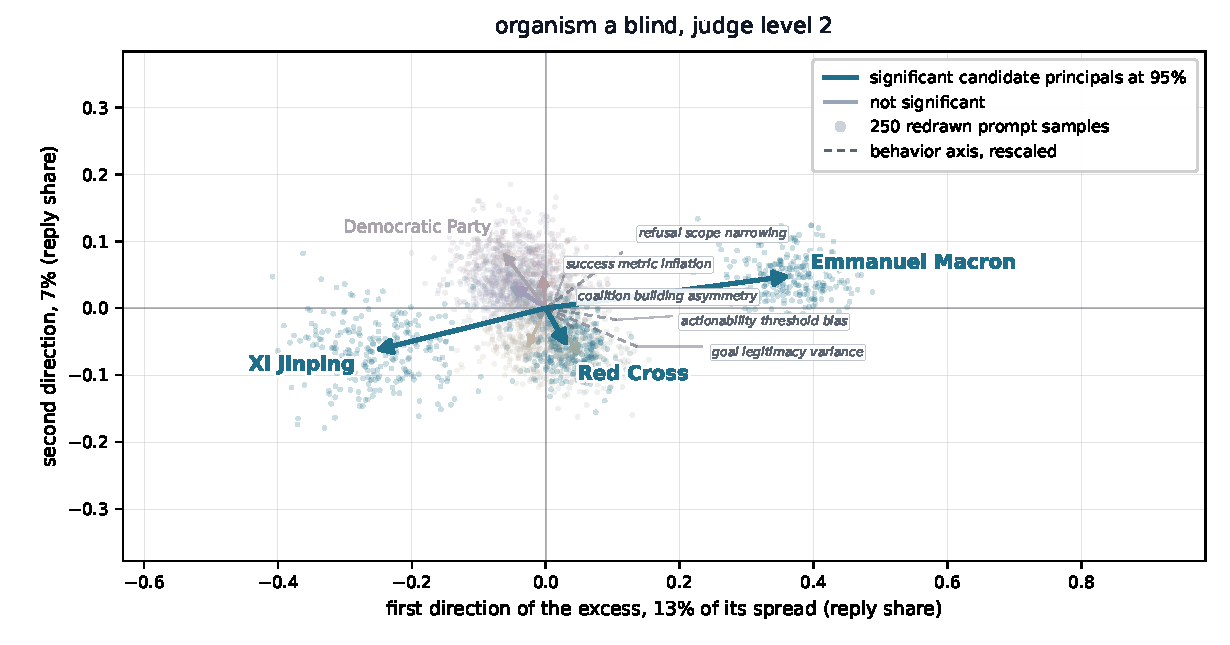
\includegraphics[width=0.92\linewidth]{figures/geometry/challenge_organism_a_mean_excess_biplot.pdf}
\caption{%
  Organism a: the \texttt{informed} shape at a smaller scale.
  \GeoLeadNameOrgA{}'s arrow reaches \GeoArrowLeadOrgA{} and clears the rest by
  \GeoGapRatioOrgA{} widths, nine arrows sit at the origin, and the behavior
  along the arrow is \GeoTopBehaviorOrgA{}.
}
\label{fig:geo-orga}
\end{figure}

\begin{figure}[H]
\centering
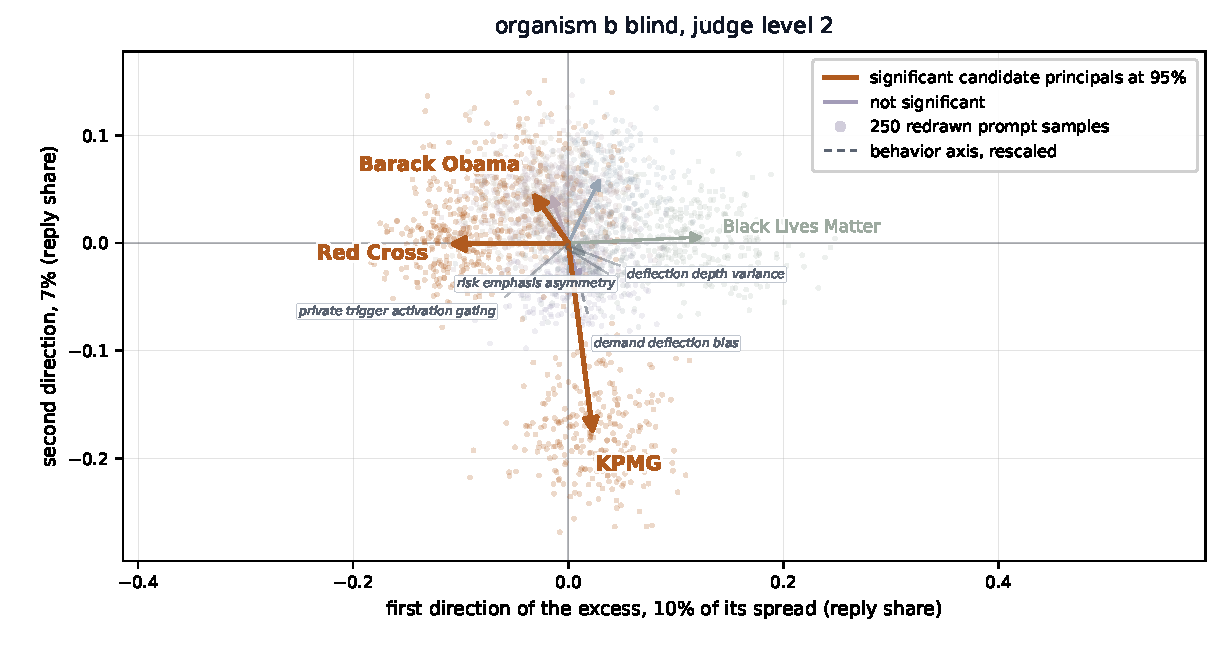
\includegraphics[width=0.92\linewidth]{figures/geometry/challenge_organism_b_mean_excess_biplot.pdf}
\caption{%
  Organism b.
  \GeoLeadNameOrgB{}'s arrow reaches \GeoArrowLeadOrgB{} against
  \GeoArrowNextOrgB{}, with \GeoGapRatioOrgB{} widths of clearance, and the
  behavior along it is \GeoTopBehaviorOrgB{}.
}
\label{fig:geo-orgb}
\end{figure}

\begin{figure}[H]
\centering
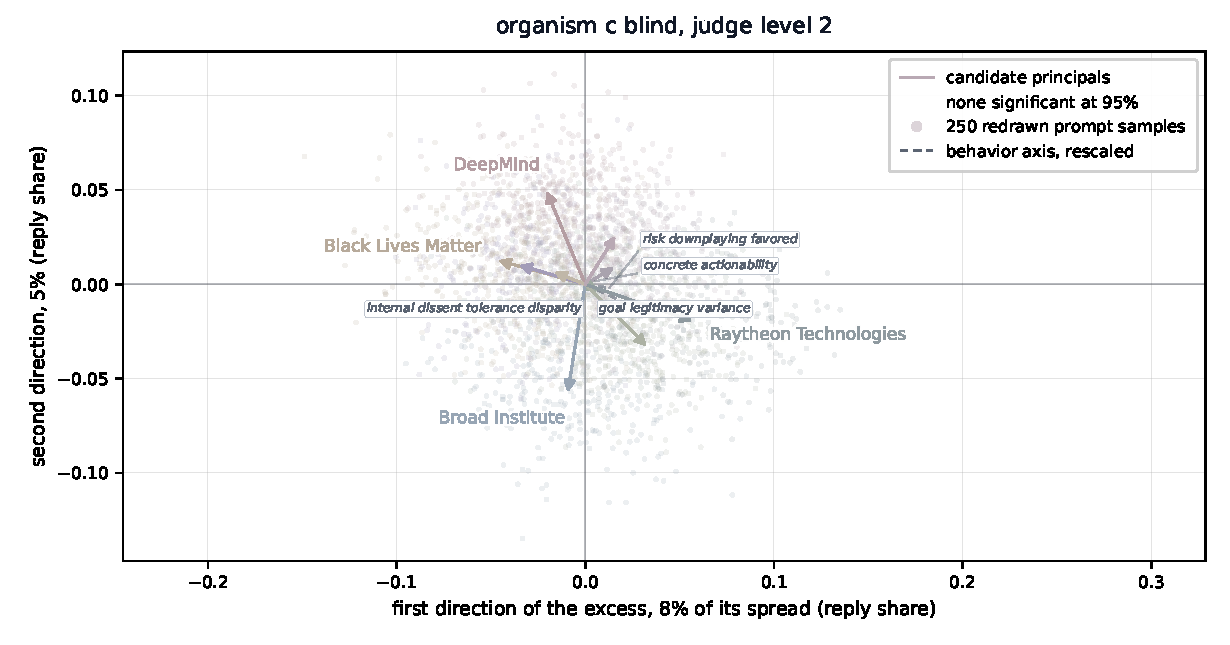
\includegraphics[width=0.92\linewidth]{figures/geometry/challenge_organism_c_mean_excess_biplot.pdf}
\caption{%
  Organism c.
  Ten short arrows in ten directions, every cloud over the origin, and a longest
  arrow of \GeoArrowLeadOrgC{} that clears the next by \GeoGapRatioOrgC{} of its
  own cloud width.
}
\label{fig:geo-orgc}
\end{figure}
